\begin{abwlearningframe}{Assessment and exam access}{\ABWInsertedPageNumber}
  \ABWRecapBar{145}{1}{Final grade: 100\% written examination.}
  \ABWRecapBar{220}{2}{Pass at least four of the six weekly assignments, plus the team assignment, to gain access to the exam.}
  \ABWRecapBar{295}{3}{The exam is individual, closed-book and handwritten; no connected devices are permitted.}

  \draw[rounded corners=8bp,fill=ABWSoftGray,draw=none]
    (55,-382) rectangle (610,-465);
  \node[anchor=west,text width=500bp,inner sep=0pt] at (78,-423)
    {{\TimesNR\fontsize{18}{21}\selectfont
      \href{\ABWCanvasAssessmentURL}{Read the Canvas announcement: grading and access conditions.}\par\vspace{4bp}
      \href{\ABWCanvasPreviousExamsURL}{Open the current Canvas module with previous and example exams.}}};

  \href{\ABWCalculatorURL}{%
    \node[anchor=north,inner sep=0pt,outer sep=0pt] at (770,-378)
      {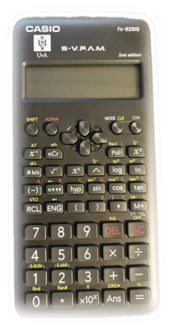
\includegraphics[height=88bp]{assets/visuals/lecture-1/casio-fx-82ms-calculator.png}};}
  \node[anchor=north,text width=250bp,align=center,inner sep=0pt] at (770,-470)
    {{\TimesNR\fontsize{13}{15}\selectfont
      \href{\ABWCalculatorURL}{SEFA: approved non-connected calculator}}};

  \node[anchor=south west,text width=550bp,inner sep=0pt] at (56,-487)
    {{\TimesNR\fontsize{9}{10.5}\selectfont\color{ABWGray}
      Course rule: \href{\ABWCanvasAssessmentURL}{Canvas assessment announcement, 31 August 2026}. Calculator product image: inherited course asset; source and reuse record pending.}};
\end{abwlearningframe}
